%
% PROJECT: Thesis for ETD, defense
%   TITLE: Approaches to Joint Base Station Selection and Adaptive Slicing in Virtualized Wireless Networks (Working Title)
%  AUTHOR: Kory Teague
% SAVE AS: KT_Thesis.tex
% REVISED: June 25, 2018

%\documentclass[12pt,dvips]{report}
%\documentclass[12pt]{report}
\documentclass[12pt,dvipsnames]{report}

\setlength{\textwidth}{6.5in}
\setlength{\textheight}{8.5in}
\setlength{\evensidemargin}{0in}
\setlength{\oddsidemargin}{0in}
\setlength{\topmargin}{0in}

\setlength{\parindent}{0pt}
\setlength{\parskip}{0.1in}

% Uncomment for double-spaced document.
%\renewcommand{\baselinestretch}{2}
%\usepackage{setspace}
%\onehalfspacing
%\doublespacing

\usepackage{cite}

\usepackage[pdftex]{graphicx}
\graphicspath{{Figures/}}
\DeclareGraphicsExtensions{.pdf,.jpeg,.png}

\usepackage{amsmath}
\usepackage{tcolorbox}
\usepackage{subcaption}
\usepackage{amsfonts}
\usepackage{bbm}
\usepackage{cleveref}
\usepackage{xargs}
\usepackage[colorinlistoftodos,prependcaption,textsize=tiny]{todonotes}

\newcommand\defeq{\mathrel{\overset{\makebox[0pt]{\mbox{\normalfont\tiny\sffamily def}}}{=}}}
\newcommand{\crefrangeconjunction}{--}
\newcommandx{\unsure}[2][1=]{\todo[linecolor=red,backgroundcolor=red!25,bordercolor=red,#1]{#2}}
\newcommandx{\change}[2][1=]{\todo[linecolor=blue,backgroundcolor=blue!25,bordercolor=blue,#1]{#2}}
\newcommandx{\info}[2][1=]{\todo[linecolor=OliveGreen,backgroundcolor=OliveGreen!25,bordercolor=OliveGreen,#1]{#2}}
\newcommandx{\improvement}[2][1=]{\todo[linecolor=Plum,backgroundcolor=Plum!25,bordercolor=Plum,#1]{#2}}
\newcommandx{\thiswillnotshow}[2][1=]{\todo[disable,#1]{#2}}

\hyphenation{vir-tu-al-iz-a-tion vir-tu-al-ized}

\begin{document}

\thispagestyle{empty}
\pagenumbering{roman}
\begin{center}

% TITLE
{\Large 
Approaches to Joint Base Station Selection and Adaptive Slicing in Virtualized Wireless Networks
}

\vfill

Kory A. Teague

\vfill

Thesis submitted to the Faculty of the \\
Virginia Polytechnic Institute and State University \\
in partial fulfillment of the requirements for the degree of

\vfill

Master of Science \\
in \\
Electrical Engineering

\vfill

Allen B. MacKenzie, Chair \\
Luiz DaSilva \\
R. Michael Buehrer \\
Mohammad J. Abdel-Rahman

\vfill

% Date, location of defense?
August 1, 2018 (TBD)\\
Blacksburg, Virginia

\vfill

Keywords: TBD
\\
Copyright 2018, Kory A. Teague

\end{center}

\pagebreak

\thispagestyle{empty}
\begin{center}

{\large Approaches to Joint Base Station Selection and Adaptive Slicing in Virtualized Wireless Networks}

\vfill

Kory A. Teague

\vfill

(ABSTRACT)

\vfill

\end{center}

\iffalse
The need for concrete examples increases when technology becomes
difficult to explain.  In documentation for computer systems
especially, we see a wide audience of field experts attempting to
comprehend documentation for computer software and hardware of which
they should only require a cursory understanding.  Additionally, as
the pace of the information age quickens we see document authors
struggle for \textit{examplia-concretes} with wide applicability, and
consistently rely on excerpts from Shakespearean literature as a
public-domain source for their various explications.

We predict the twenty-first century will be no different.  Actuarial
studies show explosion in the information industry such that four out
of five persons will be \textit{bona fide} electronic document
authors; many of those will have one or more college degrees.  We
prove through computer simulation \textsc{Machinum Simitatores} that
authors of twenty-first century literature will be affected by these
examples and will include metaphor with Shakespearean source into
their writing with increasing frequency.
\fi

\vfill

% GRANT INFORMATION

This work received support in part from the National Science Foundation via work involved with the Wireless @ Virginia Tech research group.

\iffalse
That this work received support from the Southeastern Universities
Research Association (SURA) ``Monticello Library Project'' is purely
coincidental.
\fi

\pagebreak

% Dedication and Acknowledgments are both optional
% \chapter*{Dedication}
% \chapter*{Acknowledgments}

\tableofcontents
\pagebreak

\listoffigures
\pagebreak

\listoftables
\pagebreak

\pagenumbering{arabic}
\pagestyle{myheadings}

\iftrue
\chapter{Introduction} \label{ch:intro}

Mobile carriers have seen explosive growth in both the volume of users and the demands of those users within the networks they operate.  New and evolving data-driven applications, such as audio/video streaming, social networking, and the Internet of Things have also placed increasing demand upon the networks.  In 2016, the amount of IP data handled by mobile networks exceeded 86 Exabytes; it is projected to reach almost 200 Exabytes in 2018, and 580 Exabytes in 2021~\cite{ciscoVNI2017}.  Due to this exponential growth, incremental approaches to improve the network will fail to satisfy demand.  As this growth continues to progress into the near future, new architectures like 5G and its associated technologies will be needed to keep pace with the demand.

However, deployment of these technologies and networks can be a costly, prohibitive venture.  To meet these demands requires a similar increase in capital (CapEx) and operational expenditures (OpEx).  As volumes and costs rise and margins shrink, approaches to reduce these expenditures become increasingly necessary.  Resource infrastructure sharing has been a common practice for MNOs going back to 2G and 3G networks.  First, mobile network operators (MNOs) needed to offer coverage for their users in regions where they had no infrastructure, leading to the creation of roaming agreements, eliminating the need for deploying new infrastructure in that region and reducing CapEx.  Second, by sharing passive elements of the infrastructure, such as physical sites, tower masts, power, and air-conditioning, the CapEx of deploying new backhaul and radio access networks (RANs), such as cellular base stations (BSs), has decreased~\cite{1421931}.

CapEx reductions from passive resource sharing drove an interest in resource sharing of the active elements of the network.  For example, MNOs might share RANs, core networks, BSs, antenna systems, or backhaul, which leads to reductions in both CapEx and OpEx.  The ability to share these active resources removed the necessity for network operators to own and maintain a physical network while providing actual MNO-like mobile services.  These mobile virtual network operators (MVNOs) function similarly to MNOs, but operate a virtualized wireless network (VWN) comprised of virtual resources instead of physical resources without the associated CapEx.  It has been shown that virtualization in this manner can increase overall demand satisfaction of a set of VWNs while decreasing overall cost (i.e., OpEx) by decreasing the idle capacity of the networks~\cite{MJ_CCNC_16}.

In order to take advantage of increasing virtualizable resources and competition for those resources, a specific problem must be solved: how to select the set of virtual resources to form a VWN that meets its demands with necessary or maximum demand satisfaction at minimum cost.  The solution to this problem is further complicated in the context of multiple MVNOs, each with one or more VWNs with unique demands, within a large pool of available virtual resources that can be adaptively allocated as demands shift.

This thesis addresses the topic of resource selection and adaptive slicing within cellular VWNs through the lens of a stochastic optimization problem and investigates the two approaches to efficiently reach a solution.

\section{Trends in Wireless Networking} \label{sec:netreview}

IP traffic is increasing across all types of network archetypes, and is trending to become more mobile focused.  According to the Cisco Visual Networking Index, global IP traffic will increase nearly threefold over the 2016-2021 time period, reaching 3.3 Zetabytes (ZB) annually in 2021 from 1.2 ZB annually in 2016.  Traffic across the fixed internet backbone is projected to match this threefold pace, growing from 790 Exabytes (EB) to 2.2 ZB.  However, mobile data traffic is projected to have twice the growth of fixed internet over the same period, increasing almost sevenfold from 86 EB in 2016 to 580 EB in 2021.  By the end of 2021, 17\% of global IP traffic will be mobile data or internet traffic generated by handsets, notebook cards, and mobile broadband gateways, up from 7.5\% in 2016.  More broadly, traffic from wireless and mobile devices combined will reach 63\% of total IP traffic by 2021, up from 49\% in 2016.  By 2021, smartphone IP traffic (33\% of global IP traffic) will alone outnumber PC IP traffic (25\%).  Overall, these projections show that population data use and the number of devices attached to the networks is increasing; in 2021, annual global IP traffic will reach 35 GB per capita associated with 3.5 networked devices per capita, up from 13 GB per capita and 2.3 networked devices per capita in 2016.~\cite{ciscoVNI2017}

Consumer IP traffic comprises a majority share of global IP traffic, and this share will continue to grow.  From 2016 to 2021, business IP traffic will grow at an average of 21\% compound annual growth rate (CAGR), below the growth rate of global IP traffic (24\% CAGR).  Similarly, business mobile data traffic (41\% CAGR) will lag behind that of global mobile data traffic (46\% CAGR).~\cite{ciscoVNI2017}

In both the consumer and business markets, this demand includes enormous growth in video applications, specifically that of video streaming.  By 2021, global IP video traffic will reach 82\% of all consumer internet traffic, up from 73\% in 2016.  This is represented by a threefold increase of all global IP video traffic over the period and a fourfold increase on just the internet backbone.  By 2021, internet live video streaming will account for 13\% of this video traffic, growing 15-fold over the period.  Similarly, internet video surveillance will occupy 3.4\% of internet video traffic, increasing sevenfold, and internet video to tv will increase by a factor of three and a half, growing to comprise 26\% of internet video traffic.  While these are all values for increases on the internet backbone, mobile data should see similar, but smaller, growth in these areas.  Virtual and augmented reality uses will see the largest increase, growing at a 82\% CAGR, and expected to reach a 20-fold increase between 2016-2021.~\cite{ciscoVNI2017}

The technology underlying the mobile data network needs to continue to evolve with these changing trends and growth.  The primary focus of the 5G cellular standard has been to meet these targets in an effective and robust manner.  Of specific interest is that of aggregate data rate (e.g., area capacity, the available amount of data a network can facilitate over a unit area) and edge rate (e.g., 5\% rate, the minimum data rate that can be reasonably provided to all but 5\% of users) of the network.  For 5G, the general consensus is that aggregate data rate and edge rate must be 1000x and 100x that of 4G, respectively~\cite{6824752}.  To supply these rates, several strategies are being investigated, with three primary technologies being (1) the continuing of cellular densification and offloading, (2) increased bandwidth by expanding into new spectra like Wi-Fi and millimeter wave, and (3) increasing spectral efficiency through advances such as those in massive multiple-input multiple-output (MIMO).


The first strategy is extreme densification and offloading.  By making network cells smaller, the number of active nodes increases for the same unit area.  This is a common strategy across cellular generations, and a large impetus behind the use of smaller range RANs like microcells and femtocells~\cite{4623708}.  Cell sizes have shrunk, dropping from the order of hundreds of square kilometers to now fractions of a square kilometer.  The most important benefit of cell densification is that it increases spectral reuse, which reduces the amount of users competing for the same resources.  Theoretically, since signal-to-interference ratio is maintained as the cell shrinks, such densification can be repeated indefinitely as deployments allow~\cite{6824752, 6171996}.

The second strategy is to increase bandwidth through the use of previously unused spectra such as millimeter wave (mmWave) and Wi-Fi.  Cellular networks have utilized microwave frequencies ranging from a few centimeters to about a meter in wavelength; this range has become thoroughly occupied and to generate new bandwidth would require expanding to new frequencies~[?]\change{cite (1)}.  Up to now, mmWave has been unused and in some cases unlicensed due to very poor propagation properties and high equipment costs.  However, equipment costs are falling rapidly due to technological maturation.  Further, the propagation qualities are increasingly surmountable as cell sizes shrink~[?]\change{cite (2)}.

% Cite (1) - FCC National Broadband Plan; Bandwidth Requirements for Future IMT-2000 Development
% Cite (2) - Millimeter Wave Propagation: Spectrum Management Implications; Measurement and Analysis of Propagation Mechanisms at 40 GHz; An Introduction to Millimeter-wave Mobile Broadband systems; Millimeter Wave Mobile Communications for 5G Cellular: It Will Work; Millimeter-wave Beamforming...; Millimeter-Wave Cellular Wireless Networks: Potentials and Challenges.

The third strategy involves the use of massive MIMO to increase spectral efficiency.  MIMO uses multiple transmit and receive antennas to exploit multipath signal propagation, multiplying the capacity of a given radio link.  The technology has been used for over a decade as a component of Wi-Fi before being introduced into the 3G, 4G, and 4G LTE standards~\cite{6824752}.  A new approach to be used in 5G is that of ``massive MIMO'', where the number of transmit antennas at the BS greatly outnumber the number of active users~\cite{5595728}.  For example, a given BS might have hundreds of antennas while maintaining data links for tens of users.  This provides several benefits, most importantly that of vastly improving spectral efficiency.

5G must supply these rates at much higher energy and cost efficiencies, ideally matching or exceeding the capacity increases to avoid increasing overall network energy use and OpEx.  However, technologies that have been investigated to adequately increase the capacity of the network have several major hurdles to meet in order to be implemented at the desired energy and cost efficiencies.  Massive MIMO requires the deployment of a vast number of antennas, which requires new BS architectures that have issues with scalability and cost.  Millimeter-wave is more expensive than the more mature hardware of typical cellular bands.  Decreasing cell size for cellular densification allows for smaller, cheaper BSs, but this decreased cost may not keep pace with the required number of increased deployments.  Additional measures to decrease expenditures on top of that of the aforementioned technologies is worth investigating.~\cite{6824752}

3GPP (the Third-Generation Partnership Project) is currently working on finalizing the standard for 5G implementations.  In December 2017, 3GPP froze the first half of release 15 of the 5G standard, establishing the specifications of non-standalone 5G which utilizes existing LTE networks.  It is expected that 3GPP will freeze the second half of release 15, covering 5G New Radio (5G-NR) which establishes specifications for new standalone 5G deployments, in Summer of 2018.

\section{Virtualization, Virtualized Wireless Networks, and the Networks without Borders Paradigm} \label{sec:virtualization}

One approach towards minimizing CapEx and OpEx of networks has been the utilization of resource sharing.  Resource sharing encompases the sharing of resources between multiple networks, and can take the form of \emph{passive sharing} - referring to the sharing of physical sites, tower masts, cabling, power supplies, and other components that are not actively on part of the network architecture - and \emph{active sharing} - referring to the sharing of the active network architecture itself, such as backhaul and RAN.  The practice has been utilized since 2G and 3G networks as a tool for reducing CapEx in expanding the network~\cite{1421931}.  Since then, resource sharing has become more common, where it is now available, standardized~\cite{3GPP_TS_23.251}, and implemented in many major carrier networks.  As reported by Costa-Perez et al.~\cite{6553675}, a 2010 market survey~\cite{NetSharingReport} found that over 65\% of European MNOs have deployed mobile infrastructure sharing in some form.  It was further reported~\cite{6553675} that 20\% of cells carry about 50\% of total network traffic, with the remaining 80\% of cells still causing OpEx without gain.  Through active resource sharing, networks can reduce or avoid redundant deployments and wasted capacity, reducing overall CapEx and OpEx.

The increasing prominence of active resource sharing challenges the traditional model of ownership of the various network layers and elements.  Once it became feasible for network operators to utilize resources owned and maintained by other operators, it became possible for these MNOs to operate networks primarily or only using these shared resources.  A given shared resource can be decoupled from a specific physical resource, instead enabling it to be adaptively associated with any of a given pool of qualifying physical resources as network conditions allow, establishing the shared resource as a virtual resource.  Further, virtual networks can adapt to changing network conditions, adding and removing virtual resources as capacity requirements change.  For example, a MVNO with a network of virtual resources can add additional virtual resources during the peak hours when additional capacity for end user satisfaction is needed, and removing unneeded resources during times of low demand to reduce OpEx of the network.

Other research in virtualization has been shown to improve performance in wireless networks.  Panchal and Yates~\cite{6571315} have shown on an LTE testbed that active inter-operator resource sharing improves performance of overloaded networks in terms of decreased drop probability and overloaded sectors.  Virtualized sharing methods provided further, albeit marginal, performance improvements at an increased complexity, but would be more suitable on adaptive DSA (dynamic spectrum access) based systems.  In this capacity, improved performance allows for smaller networks reducing CapEx and OpEx.  Costa-Perez et al.~\cite{6553675} found in LTE testbeds that network virtualization substrate (NVS), a suggested virtualization technique, provides improved overall throughput compared to networks without resource sharing.

\subsection{Virtualization and the Network Value Chain} \label{subsec:virtualization_valuechain}

This concept of virtualization partitions the classical wireless networking value chain, allowing for specialization of segments of the value chain into new entities such as resource providers and service providers~\cite{1421931}.  Traditional MNOs control every segment of the typical mobile network value chain (Fig. \ref{fig:ClassicNetworkValueChain}~\cite{6737248}), from spectrum to the end user.  With the introduction of virtualization techniques, MVNOs can obtain access to bulk network services available from an MNO.  This allows for MVNOs to specialize into specific formulations without the CapEx or responsibility to deploy and maintain the radio infrastructure while incurring no significant cost~\cite{6737248}.  For example, an MVNO could focus on marketing, working solely within the distribution channel to the network's customers, or the MVNO could establish itself earlier in the value chain, focusing on operating the network from the core network.

\begin{figure}
	\centering
	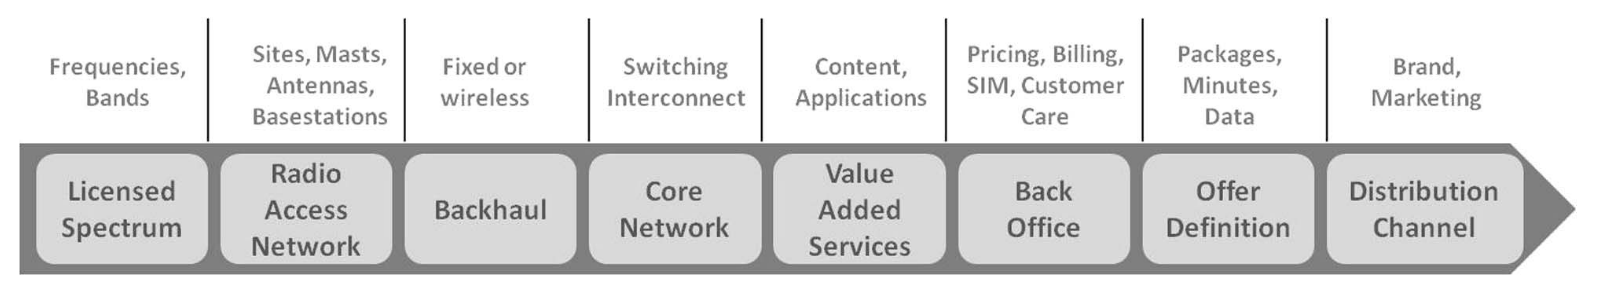
\includegraphics[width=\linewidth]{ClassicNetworkValueChain}
	\caption[Typical MNO value chain]{\small Typical MNO value chain~\cite{6737248}}
	\label{fig:ClassicNetworkValueChain}
\end{figure}

Specialization of the networks and the entities involved in the network can improve the cost efficiency of the netowork.  According to Beckman and Smith~\cite{1421931}: ``Extensive vertical integration is a characteristic of an immature product.  As the product increases in complexity, it is no longer possible to [provide] an end-to-end solution.'' In both examples, the MVNO adds value to the traditional value chain by specializing in segments (e.g., marketing or service creation) that are different from the segments (e.g., network maintenance) still handled by the owner and operator of the network resources.

By focusing on the strengths provided by virtualization, more value can be generated through specialization.  Doyle et al.~\cite{6737248} investigates the value chain with this segmentation in mind and introduces the Networks without Borders (NwoB) approach as a new service-oriented network market with a proposed new value chain (Fig. \ref{fig:NwoBValueChain}~\cite{6737248}).  The network under the NwoB approach is entirely service-oriented, where the network responds to services and connectivity is tailored for the service.  Services have a wider meaning than the voice, text, and data of a typical MNO.  Services also include that of Netflix-like or real-time video streaming, Internet-of-Things (IoT) applications, or various types of over-the-top services.  Each service would be provided by a service provider that compensates the virtual network operator operating a virtual network constructed specifically for the purpose of that service; the virtual network is the service.  Unlike an MVNO which manages resources provided to it by agreement, the virtual network operator manages slices of virtual resources from a pool of all resources as provided through resource aggregating services.

\begin{figure}
	\centering
	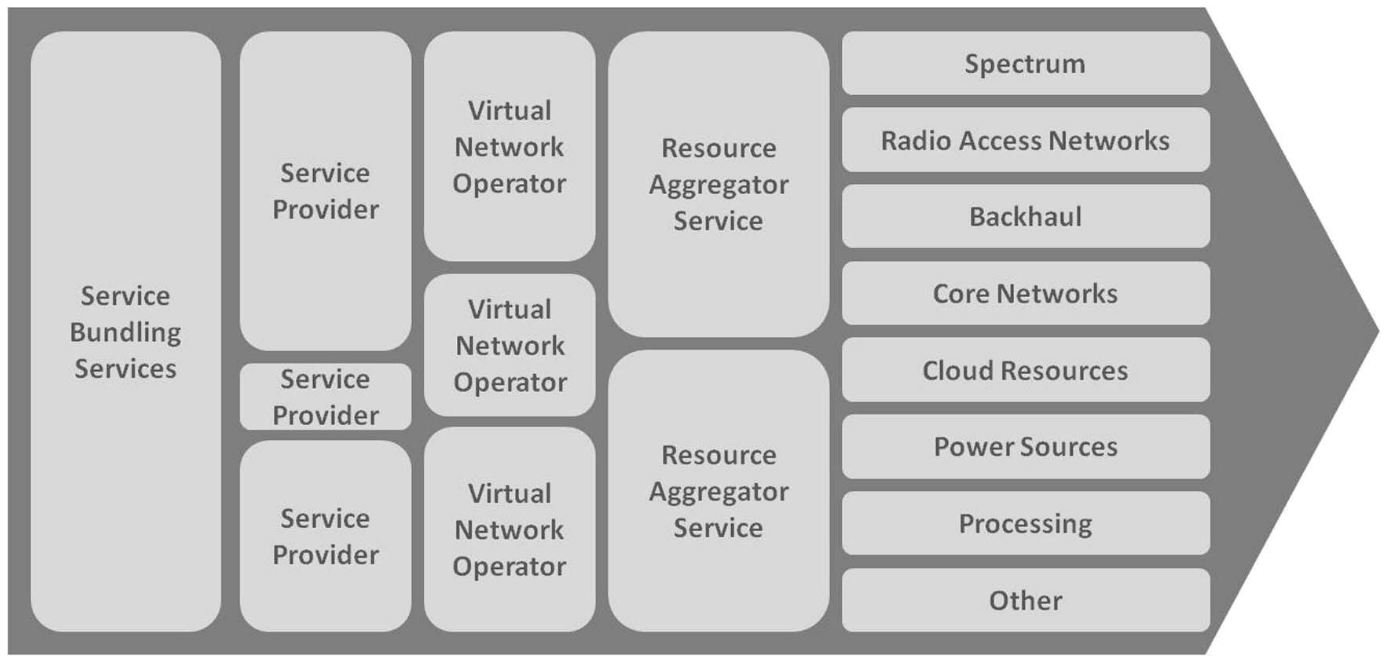
\includegraphics[width=\linewidth]{NwoBValueChain}
	\caption[Proposed network value chain under the NwoB paradigm]{\small Proposed network value chain under the NwoB paradigm~\cite{6737248}}
	\label{fig:NwoBValueChain}
\end{figure}

The benefits of this paradigm as proposed by Doyle et al.~\cite{6737248} are four-fold.  First, it provides specialization and independence for each stage, allowing service providers to focus on generating value from services provided.  Second, networks can be specialized for a service, reducing OpEx through extensive resource sharing.  Third, as resources are virtualized and pooled together, any resource (e.g., typical RAN, Wi-Fi, mmWave, raw spectrum) could be added with the pool and utilized for a network as its properties fit the network's needs.  Fourth, it lowers the barrier for entry and establishes services for new entities to fulfill.

\subsection{Virtualization Architecture in this Work} \label{subsec:virtualization_architecture}

Recognizing the critical nature of virtualization and resource allocation, this thesis develops and analyzes several methods for ... A virtualization architecture%
\unsure{Comment for the start of next sentence\\Come back to it}

This thesis utilizes a virtualization architecture~\cite{MJ_MECOMM_17} based on the NwoB paradigm presented by Doyle et al.~\cite{6737248}.  Fig. \ref{fig:VWNArchitecture}~\cite{MJ_MECOMM_17} illustrates the three primary roles in this architecture: (1) the Resource Providers (RPs), (2) the Virtual Network Builder (VNB), and (3) the Service Providers (SPs).

\begin{figure}
	\centering
	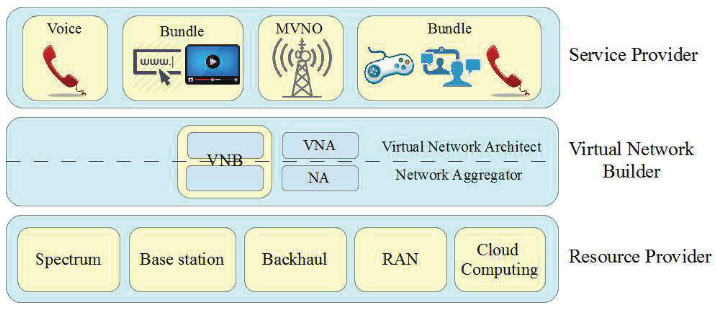
\includegraphics[width=\linewidth]{VWNArchitecture}
	\caption[VWN architecture as used in this work]{\small VWN architecture as used in this work~\cite{MJ_MECOMM_17}}
	\label{fig:VWNArchitecture}
\end{figure}

RPs deploy and maintain the physical resources that are to be virtualized and offered for use within the virtualization framework, and are the various entities that occupy the right-most column of segments (i.e., resources) in the NwoB value chain (Fig. \ref{fig:NwoBValueChain}~\cite{6737248}).  These resources can be in the form of any network-capable resource.  For example, the resources could be BSs as provided by a traditional MNO, a company-or individual-owned WLAN, femtocell access points, available licensed or unlicensed spectrum, or cloud computing.  They are any entity that offers a virtualizable resource, such as a traditional MNO, company, or individual.  Further, they maintain the resources, but also determine how the resource would be sliced and shared.  This large variety causes the underlying infrastructure of this virtualization framework to be highly heterogeneous.

The VNB acts as resource aggregator, VWN constructor, and as intermediary between SPs and RPs.  Therefore, the VNB acts as a combination virtual network operator and resource aggregator in the NwoB value chain (Fig. \ref{fig:NwoBValueChain}~\cite{6737248}).  The VNB aggregates the resources maintained by individual RPs to establish the pool of available virtual resources.  The VNB also coordinates with SPs to understand the demands of their services, and constructs VWNs tuned specifically to these demands.  By understanding the needs of the services provided by the SPs, the VNB will evaluate which virtual and virtualizable resources available from the RPs are needed to construct the optimal\footnote{In this network context, ``optimal'' is loosely defined to mean a network that provides the maximum demand satisfaction for the service provided by the SP at the minimum cost (OpEx) to be paid to the RP.  These two requirements - maximum demand satisfaction and minimum cost - are frequently contradictory and need to be balanced by the VNB.} network for the SPs' needs, coordinate with the necessary RPs to obtain access to these resources for a given wholesale (OpEx) cost, and construct the network for the SPs to operate.  Multiple VNBs can coexist, each with their potentially overlapping set of RPs from which to aggregate resources.

The SP operates very similarly to the service providers in the NwoB approach.  Primarily, an SP determines a service that they wish to provide, understands and enumerates the demands that are to be appropriately satisfied for that service, and provides the service over the VWN to their end users.  SPs can provide a wide range of services over the network.  The service could be a traditional MNO or be providing MNO-like services, such as voice calling and texting.  Services could cover specific applications, such as IoT, teleconferencing, augmented or virtual reality, or emergency services.  Other examples include traditional over-the-top services, such as Netflix-like or real-time (live) video streaming, social media (Facebook, Twitter, etc.), messaging (Skype, Groupme, etc.), or news/content feeds.  Further, an SP could also bundle several services, either through a single VWN built for the bundle, or by bundling services provided by several SPs.

Between these three entity roles, various interactions become possible.  The most common interactions are illustrated in Fig. \ref{fig:VWNArchitectureInteractions}~\cite{MJ_MECOMM_17}.  The interactions between the various entity roles are: (\emph{A}) among SPs; (\emph{B}) between the SPs and the VNBs; (\emph{C}) among VNBs; (\emph{D}) between the VNBs and the RPs; and (\emph{E}) among RPs.  It should be apparent that across each of these interactions is the imposition of costs as exchange for the transfer of services, networks, and resources.

\begin{figure}
	\centering
	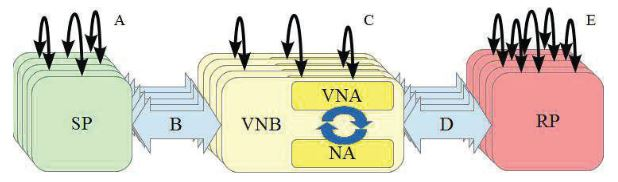
\includegraphics[width=\linewidth]{VWNArchitectureInteractions}
	\caption[Interactions between roles in the VWN architecture]{\small Interactions between roles in the VWN architecture~\cite{MJ_MECOMM_17}}
	\label{fig:VWNArchitectureInteractions}
\end{figure}

Interaction (\emph{A}) describes associations among various SPs.  This would typically occur in situations where a SP desires to bundle the services of several SPs, or when a SP wishes to utilize a specialized network operation from another SP.  Generally, this interaction would be performed manually over timescales of weeks or months.

Interaction (\emph{B}) describes associations directly between SPs and VNBs.  This would be one of the most common interactions within this framework.  This interaction is bidirectional.  In  the first direction, SPs would provide the VNB they are coordinating with the specific demands and needs for the service they are providing.  In the opposite direction, the VNB utilizes these conveyed needs and demands to construct a VWN and provide it for use to the service provider.  Ideally, this interaction is highly or entirely automated, with the interactions varying from minutes or hours to weeks or months based on the level of automation and the specifics of the interaction.  It will require optimization techniques and/or machine learning to achieve satisfactory results in this interaction.

Interaction (\emph{C}) describes associations among various VNBs.  Generally, such interactions may occur when a VNB does not have access to the appropriate virtual resources to satisfy interaction (\emph{B}) interactions.  Obvious examples include not having the necessary resources to provide adequate coverage over geographical areas or capacity in high-density environments.  These interactions would generally be performed manually over timescales of weeks or months.

Interaction (\emph{D}) describes associations between VNBs and RPs.  Similar to interaction (\emph{B}), this would be the other of the most common interactions within this framework.  It is also very important, as it establishes the mapping between the virtual and physical resources and builds the substrate that the framework is built upon.  VNBs interact with the RPs by making requests for new resources and releasing unneeded resources.  RPs interact with the VNBs by issuing updates, such as any changes to the resources in the VNBs' available pool of resources.  Updates such as these are potentially highly disruptive to the VNBs as the updates can impact a large number of VWNs managed by the VNBs.  With further similarity to interaction (\emph{B}), this interaction is highly dependent on automation; based on the level of automation, this interaction may occur over timescales of minutes or hours to weeks or months.

Interaction (\emph{E}) describes associations among various RPs.  In this interaction, various RPs establish connections with each other to facilitate proper mapping of physical resources to virtual through the use of quality of service (QoS) parameters that define the abstracted resources.  For example, a small-scale RP containing only an individual-owned femtocell could connect with a larger RP via this interaction so that the resource within the small-scale RP is visible for association with a VNB over interaction (\emph{D}) as handled by the larger RP.  These interactions could take seconds to weeks depending on the complexities of the RPs, their resources, and the amount of human involvement.

Other work has been completed using this architecture.  Mohammad et al.~\cite{MJ_CCNC_16} constructed several resource allocation models, including one-stage programs, two-stage programs, and a one-stage stochastic program, to investigate the efficacy of this virtualization architecture upon a preexisting set of resources.  The implementation focused on interaction (\emph{B}) from the perspective of the VNB, and showed that virtualization decreased the cost and idle capacity of the networks and increased demand satisfaction of the networks.

Cardoso et al.~\cite{MJ_MECOMM_17} expanded on this work by introducing a two-stage stochastic program to optimize interaction (\emph{B}).  The two-stage stochastic resource allocation similarly reduces cost and idle capacity of the VWN compared to the network without sharing.  However, no direct comparisons are made with the non-stochastic programs tested by Mohammad et al.~\cite{MJ_CCNC_16}.

Marcela et al.~\cite{pittir33631} utilized this architecture from an economics perspective.  Using a matching markets framework, they investigated the interaction of association between SPs and VNBs, such as the methods for how SPs indicate their needs and how VNBs indicate their VWN capabilities, and the fees that SPs will pay to partner for a VNB.  Marcela expanded on this work in her Ph.D. dissertation~\cite{pittir33130}.%
\unsure{Still reading/parsing these papers.  Double check.}

The focus of this thesis is on optimization approaches largely in the context of interaction (\emph{B}).  This problem involves establishing how SPs convey the demands needed by the VNB to construct an optimal VWN for the service provided by the SP.  Further, the construction of the optimal VWN is sought within a short amount of time so that interaction (\emph{B}) can be completed over shorter timescales (e.g., minutes or hours) instead of longer (e.g., days, weeks, months).  With an optimal VWN in mind, construction of the VWN is inherently an optimization problem, and the seeking of expedient solutions lays within the study of optimization.

\section{Review of Optimization Methods} \label{sec:optreview}

%\unsure{In this thesis, the problem ... is approached by...}%
%\unsure{Restructure to get rid of first-person ``I''?}%
In this thesis, I approach the problem of the creation of optimal networks by the VNB that satisfy the specific demands of SPs using a pool of resources provided by a set of RPs.  This is naturally a form of optimization problem, in which some objective function is either minimized or maximized.  At it's most basic, optimization techniques (e.g., linear programming, integer programming) will find the set of input parameters that minimize or maximize a single decision variable - the value of the objective function - in context of a set of constraints.  More complex optimization problems can solve for multiple decision variables by establishing weights based on their relative importance within the objective function.

\subsection{Stochastic Programming}	\label{subsec:optreview_stoch}

Standard linear and integer programming requires complete, certain knowledge of all parameters that affect the functions or model being optimized (i.e., the model's parameters and functions must be deterministic).  Communications, especially wireless communications, can be highly non-deterministic as the communication channel introduces a large amount of uncertainty.  Stochastic programming provides a powerful mathematical tool to handle optimization under such uncertainties.

Stochastic programming has been recently exploited to optimize resource allocation in various types of wireless communications operating under uncertainties.  Abdel-Rahman et al.~\cite{MJ_CCNC_16} exploit stochastic optimization within the framework of the virtualization architecture presented in Section \ref{subsec:virtualization_architecture} to minimize the cost of resource allocation by introducing probabalistic QoS guarantees.  Cardoso et al.~\cite{MJ_MECOMM_17} expand on that work by introducing a second stage to balance maximizing demand satisfaction while minimizing cost.  Abdel-Rahman and Krunz~\cite{MJ_TW_13} utilize stochstic programming for resource allocation in DSA networks considering satisfaction of link demand as a stochastic constraint.  Abdel-Rahman et al.\cite{MJ_WCNC_16} propose a stochastic optimization formulation to optimally orchestrate LTE-U networks that utilize Wi-Fi access points considering stochastic QoS guarantees.  Abdel-Rahman et al.~\cite{MJ_DySPAN_15} utilize stochastic optimization for resource allocation in opportunistic LTE-A networks considering the probability of rate demand satisfaction for end users.  Soltani et al.~\cite{CC_OFDMA} utilize stochastic optimization as a tool for resource allocation tasks for OFDMA-based cognitive radios considering interference from primary user systems.  Atawia et al.~\cite{CC_video} utilize predictive resource allocation techniques, which include the use of stochastic optimization, for improving energy-efficient video streaming for mobile end-users, such as those riding buses and trains.

Introducing stochastic parameters and constraints allows the optimization model to consider probabilities within the optimization.  In the case of resource allocation in networks, it may be possible to allocate enough resources to satisfy all end-user demand.  Such an optimization may require too many resources to be economical considering the law of diminishing returns, with the solution being cost prohibitive.  It is much cheaper to solve such that 95\% or 99\% of demand is satisfied, leaving the remainder as unfortunate momentary edge cases.

However, standard linear programming techniques cannot solve models with stochastic parameters.  Stochastic programming therefore requires converting the stochastic program into its deterministic equivalent program (DEP) which replaces all stochastic variables with deterministic variables~\cite{stochprogramming}.  The process of forming a DEP from a stochastic program involves converting each stochastic variable into a set of all possible scenarios and scenario probabilities.  These scenarios and scenario probabilities are present within the model as a new dimension and weight for the now-deterministic variable.  To fully encapsulate the stochastic variable, the deterministic equivalent variable may be composed of an uncountably\unsure{Is it, or is it just countable? Maybe the textbook talks of this.}~infinite set.

Resource allocation problems are typically some form of integer programming - in which all decision variables (unknowns) are integers - or mixed integer programming - in which some decision variables (unknowns) are integers.  Both integer and mixed integer programs are considered generally NP-hard and thereby intractable\info{The set cover problem, which the optimization program is a form of, is provably NP-complete.\\Therefore, it is NP-hard.~\cite{Korte:2007:CombOptimization}}.  As the programs increase in scope, they become enormously more computationally complex to solve; accounting for the scenarios of the previously stochastic variables further increases this complexity.  Finding the optimal solution may require more time than is feasible; in the worst case, these problems run in exponential time complexity.

\subsection{Metaheuristic Approaches} \label{subsec:optreview_meta}

The use of heuristic or metaheuristic algorithms can provide close-to-optimal solutions in much better time.  Examples include hill climbing, simulated annealing, ant colony optimization, and particle swarm optimization.  Each of these approaches are iterative techniques.

Hill climbing starts with an arbitrary solution and makes incremental changes to variables, finding a new solution.  If the new solution is more optimal than the previous, the new solution is iterated upon.  This continues until no further improvements are made.  Hill climbing will only find the local maximum close to the initial arbitrary solution, and is best in convex problems where the only local maximum is guaranteed to be the global maximum.

Simulated annealing is inspired by the process of annealing found in metallurgy, where metal is heated to the point where atoms can migrate, reducing defects in the crystalline structure.  In simulated annealing, the model has some notion of internal energy of the system to be minimized, temperature, and discrete states with one being an initial state.  On each iteration, the temperature drops, or cools, slightly, and the system selects a new state that neighbors the current one, and switches to the new state with a probability dependent on the temperature and the energies of the current and new state.  For temperatures greater than zero, the system can transition to a state with higher energy (i.e., that is less optimal) to better investigate the search space.  As temperature drops, the system's energy will tend to drop.  When the temperature reaches zero, the system will only transition to states of lower energy (i.e., that are more optimal), reducing to the hill climbing algorithm.

Ant colony optimization is inspired by the behavior of ants.  A colony of ants move around independently trying to find food, laying pheromones on the taken path.  Upon crossing paths, ants have a probabilistic chance to follow the new path based on the strength of the pheromones of the new and old paths.  Over time, pheromones evaporate, and paths less taken will weaken.  Longer paths, since they take longer to traverse and will be reinforced less often, will also weaken.  This has benefits over approaches like simulated annealing because it adapts in real time.

In particle swarm optimization, a number of candidate solutions, called particles, are created that move semi-chaotically.  In each iteration, every particle will move according to its velocity.  Each particle has it's best known position, and it's velocity updates in a way guided by their own best known position and the swarm's best known position.  This allows a large portion of the search space to be investigated, investigate candidate solutions to explore for regions containing local maxima until it settles to exploit and find the best found local maxima.

%\unsure{Restructure to get rid of first-person ``I''?}%
In this thesis, I utilize a genetic algorithm as an approach for optimization.  A genetic algorithm is a form of evolutionary algorithm, a set of algorithms which are inspired by biological evolution and natural selection.  Each iteration is called a \emph{generation} and is composed of a number of candidate solutions called \emph{individuals}.  Each individual is defined by a \emph{chromosome} which details the specific candidate solution.  During each generation, every individual is evaluated on its \emph{fitness}, a function dependent on the individual's chromosome; the higher the individual's fitness, the more optimal the individual.  Individuals called \emph{parents} are then randomly selected to pass their chromosome onto the next generation in a process called \emph{selection}; in selection, more fit individuals are more likely to be selected.  With a certain probability, groups of parents will undergo \emph{crossover} and exchange the data contained within their chromosomes to form new \emph{children} that are a mixture of the parents; if mixing does not occur, the parents are cloned into the next generation as children.  Then, individual bits within the children's chromosomes have a chance to flip, or \emph{mutate}.  The resulting children from crossover and mutation form the entire next generation.

Since chromosomes from fitter individuals are more likely to pass on to subsequent generations, generations gradually become fitter.  Through crossover, fit chromosomes may combine to form fitter children that proliferate; less fit children are often also formed, but are generally not selected for later generations.  Mutation introduces diversity into the generations, which expand the exploration of the search space.  More details, including that of implementation and variants, will be expanded upon in Section \ref{sec:ga}.

Genetic algorithms have been used previously as approaches for simplifying constraints of large, complex stochastic optimization problems.  Cui et al.~\cite{7257198} used a genetic algorithm where each chromosome defined a subproblem of the larger optimization problem, and the fitness was evaluated by solving the subproblem with linear programming optimization methods.  Hybrid approaches, such as the one used by Cui et al.~\cite{7257198}, and other effective metaheuristic algorithms (e.g., ant colony optimization, particle swarm optimization, neural networks and machine learning) are worth investigating in the context of the posed VWN architecture, but beyond the scope of this thesis.

\section{Thesis Objective} \label{sec:objective}

The objective of this thesis is to develop two approaches of joint resource allocation to construct a set of a VWNs and adaptively slice the selected resources to the individual VWNs.  A model will be presented as the context for these approaches, expanding upon the VWN architecture proposed in Section \ref{subsec:virtualization_architecture}.  The validity of this model will be restricted to the scope of cellular networks using generic base stations as its resources with perfect connections to demand points within range.  The two proposed approaches will be performed within the VNB, and evaluated in four cases that differ in the resources provided by the RPs and service demands to be satisfied by the SPs.  Accordingly, the efficacy of these approaches will be measured primarily by the optimality of the solutions, such as cost and network service demand satisfaction, and the run time, providing the VNB with a sufficient solution in a reasonable amount of time.

\section{Thesis Outline} \label{sec:outline}

This thesis is organized as follows.  Chapter \ref{ch:intro} establishes the motivation for investigating resource selection for virtual network construction.  Chapter \ref{ch:intro} also presents the associated background information and literature review regarding virtualization, wireless networks, and optimization.  Chapter \ref{ch:vnbmodel} defines the model used for the resource allocation methods explored in this thesis.  Further, Chapter \ref{ch:vnbmodel} also details the two-stage stochastic optimization problem which optimally performs resource selection and slicing as a basis of approaches presented within this work. Chapter \ref{ch:approaches} establishes the two approaches investigated to provide solutions to the optimization problem posed in Chapter \ref{ch:vnbmodel}: a sampled Deterministic Equivalent Program which solves the problem as a whole and a genetic algorithm that simplifies the problem by providing an estimated optimal resource selection.  Chapter \ref{ch:testsim} tests these two approaches by presenting four data sets that mimic real world cellular networks and evaluates the results.  Chapter \ref{ch:conc} contains the conclusions and proposed future work in this area.
\fi

\iftrue
\pagebreak
\chapter{Virtual Network Builder Model} \label{ch:vnbmodel}

This chapter establishes the mathematical foundation for the work completed in this thesis.  First, a geographic model is presented, defining an area of interest, the pool of resources maintained by the RPs for use by the VNB, a characterization for service demand communicating the needs for the SPs' VWNs, and the SPs' end users to be satisfied.  Second, a two-stage stochastic program utilizing this model is proposed to solve the posed problem of resource selection and adaptive slicing for use in VWN construction within the VNB.

\improvement{Go through chapter notes, and break them down to where and what.}%
\textit{This chapter discusses the model upon which the approaches that are run within the VNB are defined.  It discusses the assumptions that the VNB runs within and lays out the optimization problem that the VNB is tasked with solving.}

\textit{Begin breaking down the model used as the basis for the work.  Start with a lead in, then start defining the model in the first subsection.  Expound on some of the definitions and descriptions that I moved past in the conference paper (perhaps describing the SSLT model more fully).  Make sure that the definitions and work are generalized for writing about a constructed VWN (or constructed VWNs, depending on the terminology I intend to use) for multiple RPs and SPs.}

\section{Network Area Definitions} \label{sec:networkdefs}

\textit{Change ``we''s to ``I''s or alternate voice.  Expand SSLT description: a mention of $\rho^S$, the specific autocorrelation which is dependent on $\omega_{\max}$, the differences between my implementation and Lee's, and any other pertinent information (review ``Lee, Zhou, and Niu'' \cite{6554749}).  Expound directly on the assumption I make that demand has a perfect connection within range and no connection out of range (i.e., $u_{ms} = 1$ if DP m is less than or equal to $b_s$ distance from BS s and $u_{ms} = 0$ otherwise).  Expound on nonstationary PPP procedure; provide more information laying out the process, and include the possibility of generating a set number of demand points if desired - this does alter the PPP slightly, in that the PPP no longer has a specific overall density of points, but it does maintain the structure of the overall density function, scaled to a desired degree.  Ensure equations are spaced well for full page, and devoid of unnecessary horizontal and vertical spacing (from when the conference paper was trimmed).  A figure demonstrating continuous SSLT model and a possible scenario of demand points would be appropriate here.  Improve on the overall wording/phrasing regarding the capability for multiple RPs and SPs to be present; that is BSs come from the overall pool of RP resources which the VNB is selecting to build its VWNs of interest, then slices those selected resources into forming the specific, individual VWNs for each SP.  When referring to ``Problem''s (e.g., Problem 1 from section \ref{sec:stochopt}), refer to the equations that make up that problem; see first reference of Problem 1 in Chapter \ref{ch:approaches} for reference.}

We consider a geographical area of width $X$ (m) and length $Y$ (m) that contains a set $\mathcal{S} \defeq \left\{1,\, 2,\, \ldots,\, S\right\}$ of BSs available to be leased to the VNB by a set of $\mathcal{N} \defeq \left\{1,\, 2,\, \ldots,\, N\right\}$ RPs.  The rate capacity of BS $s \in \mathcal{S}$ is denoted by $r_s$, its cost is denoted by $c_s$, and its coverage radius is denoted by $b_s$.

A Service Provider (SP) seeking a virtualized wireless network from the VNB is assumed to know the distribution of traffic demand within the region the VWN would cover.  It has been shown that a log-normal distribution or a mixture of log-normal distributions can approximate traffic demand in real-world cellular networks~\cite{686105, 5936263}.  It has also been shown that traffic distribution is spatially correlated~\cite{5936263, eigenplaces}.  We model the spatial traffic demand of a single SP using a similar, continuous form of the SSLT (Scalable, Spatially-correlated, and Log-normally distributed Traffic) model as proposed by Lee, Zhou, and Niu~\cite{6554749}.

To generate this spatial distribution over the area of consideration, an initial Gaussian field, $\rho^G = \rho^G\left(x,\, y\right),\, x \in \left[0,\, X\right],\, y \in \left[0,\, Y\right]$, is generated by
\begin{equation}
\rho^G\left(x,\, y\right)=\frac{1}{L} \; \sum_{l=1}^L \cos\left(i_lx+\phi_l\right) \; \cos\left(j_ly+\psi_l\right)
\end{equation} \label{eq:rhoG}
\noindent where $\mathcal{L} \defeq \left\{1,\, 2,\, \ldots,\, L\right\}$ is a set of the products of two cosines with angular frequencies $i_l,\, j_l\, \sim \mathcal{U}\left(0,\, \omega_{\max}\right),\, l \in \mathcal{L}$ and phases $\phi_l,\, \psi_l\, \sim \mathcal{U}\left(0,\, 2\pi\right),\, l \in \mathcal{L}$.  As $L$ increases, $\rho^G$ approaches a Gaussian random field with a spatial autocorrelation dependent on $\omega_{\max}$ according to the central limit theorem.

The approximate Gaussian distribution $\rho^G$ is then normalized to a standard normal distribution.  The final log-normal distribution, $\rho = \rho\left(x,\, y\right), x \in [0,\, X], y \in [0,\, Y]$, is determined by assigning location and scale parameters
\begin{equation}
\rho\left(x,\, y\right) = \exp\left(\frac{\sigma}{\sqrt{\text{Var}\left(\rho^G\right)}} \; \rho^G\left(x,\, y\right)+\mu\right)
\end{equation} \label{eq:rhoLN}
\noindent where $\text{Var}\left(\rho^G\right)$ is the variance of $\rho^G$.

$\rho\left(x,\, y\right)$ can be sampled over the space into individual pixels as per Lee with each pixel's value indicating the number of homogeneous demand points within the pixel~\cite{6554749}.  In contrast, we allow $\rho\left(x,\, y\right)$ to provide a continuous, spatially-correlated log-normal distribution depicting the demand density over the region for the SP.

Let $\mathcal{M} \defeq \{1,\, 2,\, \ldots,\, M\}$ be the set of the SP's demand points seeking to connect to the VWN; the value of total traffic demand at each point is denoted by $d_m$.  Further, let $u_{ms} \in [0,\, 1],\, m \in \mathcal{M},\, s \in \mathcal{S}$, represent the normalized capacity (with respect to $r_s$) of BS $s$ at point $m$, i.e., the normalized maximum rate that a user can receive at point $m$ from BS $s$.  $u_{ms} = 0$ when $m$ is outside the coverage area of $s$ and $u_{ms} = 1$ when $m$ is within a small distance of $s$.  The specific position of the points in $\mathcal{M}$, and therefore the values of $u_{ms}$, is determined via a non-stationary 2D Poisson point process (PPP) with $M$ points using the demand field, $\rho$, as the spatial intensity function.  To generate this non-stationary PPP, we use an acceptance-rejection method.  Each point of a stationary PPP with an intensity of $\rho_{\max} = \max_i\rho\left(x_i,\, y_i\right)$ is retained with probability $\frac{\rho\,\left(x_i,\, y_i\right)}{\rho_{\max}}$, where $x_i$ and $y_i$ are the x- and y-coordinates of the $i^{th}$ point of the stationary PPP.

We assume that a BS $s \in \mathcal{S}$ can be allocated between multiple demand points, and $\delta_{ms} \in [0,\, r_s],\, m \in \mathcal{M},\, s \in \mathcal{S}$, represents the rate of BS $s$ that is allocated to point $m$.

Throughout this paper, stochastic variables will be differentiated from deterministic variables with a tilde ($\sim$) placed above the symbol.

\section{Stochastic Optimization} \label{sec:stochopt}

\textit{Replace ``we''s to ``I''s or find alternate wording/tense/voice.  Ensure equations are spaced appropriately for full page column and that there are no unnecessary vertical or horizontal spacing.  Expounding on the various components of the stochastic optimization problem might be worthwhile.  Might be worthwhile to also mention that the stochastic nature of this specific formulation is limited to handling stochastic demand point locations.  As with \ref{sec:networkdefs}, modify wording and phrasing accordingly to accommodate the possibility for multiple RPs and SPs in the model.  When referring to ``Problem''s (e.g., Problem 1 from section \ref{sec:stochopt}), refer to the equations that make up that problem; see first reference of  Problem 1 in Chapter \ref{ch:approaches} for reference.}

We formulate the presented problem as a two-stage stochastic optimization problem.  We introduce $z_s, s \in \mathcal{S}$ as a binary decision variable defined as
\[ z_s \defeq
	\begin{cases}
		1,& \text{if BS $s$ is selected for the created VWN,}\\
		0,& \text{otherwise.}
	\end{cases}
\]

To balance the interest of maximizing demand satisfaction against minimizing cost, we introduce the positive real number $\alpha$ as a weighting coefficient between the two stages.

\vspace{3mm}
\begin{tcolorbox}[title = Problem 1 (Two-Stage Stochastic Optimization Problem)]
\begin{align}
& \underset{\left\{z_s,\, s \in \mathcal{S}\right\}}{\text{minimize}} \left\{ \sum_{s \in \mathcal{S}} c_s \; z_s + \alpha \mathbb{E}\left[ h\left( z,\, u \right) \right] \right\} \label{eq:P1S1}\\
& \text{subject to:}  \nonumber \\
& \hspace{0.4in} z_s \in \{0, 1\}, \forall s \in \mathcal{S} \label{eq:P1S1C1}
\end{align}
where $h(z, u)$ is the optimal value of the second-stage problem, which is given by:
\begin{align}
& \underset{\left\{\substack{\delta_{ms}, m \in \mathcal{M}, s \in \mathcal{S}}\right\}}{\mathrm{minimize}} \left\{ - \sum_{m \in \mathcal{M}} \sum_{s \in \mathcal{S}} \delta_{ms} \; \tilde{u}_{ms} \right\} \label{eq:P1S2}\\
& \text{subject to:}  \nonumber \\
& \hspace{0.4in} z_s = \mathbbm{1}_{\left\{\sum_{m \in \mathcal{M}} \delta_{ms} > 0\right\}}, \forall s \in \mathcal{S} \label{eq:P1S2C1}\\
& \hspace{0.4in} \sum_{s \in \mathcal{S}} \delta_{ms} \; \tilde{u}_{ms} \leq d_m, \forall m \in \mathcal{M} \label{eq:P1S2C2}\\
& \hspace{0.4in} \sum_{m \in \mathcal{M}} \delta_{ms} \leq r_s, \forall s \in \mathcal{S}. \label{eq:P1S2C3}
\end{align}
\end{tcolorbox}

The first stage objective function (\ref{eq:P1S1}) minimizes the total cost of the selected network with respect to that network's ability to satisfy the demand contained within the region.  The second stage objective function (\ref{eq:P1S2}) maximizes demand satisfaction by maximizing the total demand allocated to the resources comprising the network, as specified by $\delta_{ms}$ as the decision variable of the second stage.

Constraints (\ref{eq:P1S1C1}), (\ref{eq:P1S2C1}), and (\ref{eq:P1S2C3}) implement the defined ranges and values of the decision variables $z_s$ and $\delta_{ms}$, with (\ref{eq:P1S2C1}) ensuring that demand is allocated only to selected resources.  For constraint (\ref{eq:P1S2C1}), $\mathbbm{1}_{\{*\}}$ is defined by
\[ \mathbbm{1}_{\{*\}} \defeq
	\begin{cases}
		1,& \text{if condition $\{*\}$ is true,}\\
		0,& \text{otherwise}.
	\end{cases}
\]

Constraint (\ref{eq:P1S2C2}) ensures a demand point $m \in \mathcal{M}$ is not allocated more resources than it demands.
\fi

\iftrue
\pagebreak
\chapter{Approximation Approaches} \label{ch:approaches}

\improvement{Go through chapter notes, and break them down to where and what.}

\textit{Replace with introduction paragraph to this chapter.  This chapter lays out the two major approaches I am using in this thesis: the sampled DEP and genetic algorithm, and the foundation those approaches are built on.  These approaches are built on the stochastic optimization problem as laid out in \ref{sec:stochopt}, and meant to provide a solution (i.e., the DEP) or an estimate (i.e., the sampled DEP and genetic algorithm) as the original problem is not directly solvable.}

\textit{In this chapter, I work on defining the approximation approaches used in my work.  Lead in to discussing the need to approximate the stochastic optimization problem from section \ref{sec:stochopt} to adequately solve my work, then introduce the two approaches I used to approximate the optimization problem: the DEP/its sampling/generalized post-selection slicing and the genetic algorithm as a selection method.}

\section{Deterministic Equivalent Program} \label{sec:dep}

\textit{Replace all ``we''s with ``I''s or with alternate phrasing/tense/voice.  When referring to ``Problem''s (e.g., Problem 1 from section \ref{sec:stochopt}), refer to the equations that make up that problem; see first reference of Problem 1 in Chapter \ref{ch:approaches} for reference.}

\textit{Introduce the idea of a DEP as an approach for solving the original stochastic problem.  Present the solved problem here in the form of the true deterministic equivalent program - as in, it is actually an equivalent to the original stochastic problem - with all the necessary expansions and additional variables.  Focus on how this formulation no longer includes any stochastic variables and is purely deterministic.  Mention that the trade off is that the deterministic variables are part of a infinitely large set of potential scenarios.}

In order to solve the two-stage stochastic optimization formulation (Problem 1, \cref{eq:P1S1,eq:P1S1C1,eq:P1S2,eq:P1S2C1,eq:P1S2C2,eq:P1S2C3}), we need to convert it to a deterministic equivalent program (DEP) that does not contain any stochastic variables (only deterministic variables)~\cite{stochprogramming}.

Let $\Omega$ be defined as the sample space, i.e., the set of all scenarios.  Let $\hat{\Omega} \defeq \{1,\, 2,\, \ldots,\, O\}$ be a discrete set containing sampled scenarios.  The probability a given scenario $\omega \in \hat{\Omega}$ occurs is denoted by $p^{(\omega)},\, \omega \in \hat{\Omega}$, where $\sum_{\omega \in \hat{\Omega}} p^{(\omega)} = 1$.  Variables that are dependent on the scenario are shown with a superscript ($\omega$) with the specific scenario it is dependent on indicated by $\omega$.

\vspace{3mm}
\begin{tcolorbox}[title = Problem 2 (Deterministic Equivalent Program of Problem 1)]
\begin{align}
& \underset{\left\{ \substack{
	z_s,\, \delta_{ms}^{(\omega)},\\
	s \in \mathcal{S},\, m \in \mathcal{M},\\
	\omega \in \hat{\Omega}} \right\}} {\text{minimize}}
\left\{ \sum_{s \in \mathcal{S}} c_s \; z_s - \alpha \sum_{\omega \in \Omega} p^{(\omega)} \left( \sum_{m \in \mathcal{M}} \sum_{s \in \mathcal{S}} \delta_{ms}^{(\omega)} \; u_{ms}^{(\omega)} \right) \right\} \label{eq:P2}\\
& \text{subject to:}  \nonumber \\
& \hspace{0.4in} \sum_{s \in \mathcal{S}} \delta_{ms}^{(\omega)} \; u_{ms}^{(\omega)} \leq d_m,\, \forall m \in \mathcal{M},\, \forall \omega \in \hat{\Omega} \label{eq:P2C1}\\
& \hspace{0.4in} \sum_{m \in \mathcal{M}} \delta_{ms}^{(\omega)} \leq r_s \; z_s,\, \forall s \in \mathcal{S},\, \forall \omega \in \hat{\Omega} \label{eq:P2C2}\\
& \hspace{0.4in} z_s \in \{0,\, 1\},\, \forall s \in \mathcal{S}. \label{eq:P2C3}
\end{align}
\end{tcolorbox}

The objective function (\ref{eq:P2}) combines both objective functions (\ref{eq:P1S1}) and (\ref{eq:P1S2}) of the initial formulation into a deterministic form.  Constraints (\ref{eq:P2C1}) and (\ref{eq:P2C2})	ensure demand is not overallocated and is only allocated to selected resources and within capacity for all scenarios.

Problem 2 provides an equivalent deterministic form of Problem 1 for the (finite) sampled state space, $\hat{\Omega}$, containing $O$ scenarios.  With sufficiently large $O$, $\hat{\Omega}$ approaches a tight approximation of the original sample space.  Within each scenario $\omega \in \hat{\Omega}$, the SSLT demand field $\rho$ is sampled to provide a set of $M$ discrete demand points.  Each sampling of $\rho$ is generated by creating a non-stationary 2D PPP with $M$ points as described in Section \ref{sec:networkdefs}.

\subsection{Sampling Approaches} \label{subsec:dep_sampling}

\textit{As the infinitely large set of scenarios renders the problem unable to be solved, it needs to be sampled into a finite set to be solved.  Present the structure and nomenclature used to imply a sampled set of scenarios, and describe the structure of how the scenarios are sampled into a truncated set.  Might be worth mentioning that there are other methods that might be better for sampling beyond the completely random sampling approach I am using.  Worth consideration?}

\subsubsection{Sample Average Approximation} \label{subsubsec:dep_sampling_saa}

\textit{At what point is the sampling enough?  As the set of scenarios considered within the sampled DEP increases, it more closely compares to the original DEP and the stochastic optimization problem, but it also becomes increasingly difficult to solve as the number of scenarios considered increases.  So, it is beneficial to understand that a certain known number of scenarios provides a reasonably tight - what does reasonable mean? - solution to the original DEP to avoid being unnecessarily computationally expensive to solve.  Finding this minimum necessary number of scenarios can be done via a sample average approximation (SAA) analysis, which should not be too complicated to do.}

\subsection{Adaptive Slicing} \label{subsec:dep_slicing}

\textit{Now that we have a (close) approximation to the DEP and the original stochastic optimization problem, we have a method for deriving the minimum cost BS selection and adaptive slicing for the desired VWN.  However, this selection is overly time consuming to constantly run, and the BSs selected for the VWN(s) by the VNB are fairly constant, so all that is needed is to dynamically (read: adaptively) slice the selected BSs to the various SPs.  To do this, we simplify the sampled DEP such that it has only one scenario - ostensibly, the current scenario in time - and the BSs selected set to be a constant rather than a decision variable.  The resulting problem is a single stage linear program that is much simpler to solve.  This is used to adaptively slice resources to the demand.}

After the solution to the sampled DEP of Section \ref{subsec:dep_sampling} has been found, the VNB has determined the joint BS selection that forms the VWN and a proposed resource slicing of considered possible scenarios, $\hat{\Omega}$, that allocates the resources to the SP's demand points.  Since $O$ is not infinite, any given scenario present in the formed VWN is unlikely to be an element of $\hat{\Omega}$.  Further, as demand points move between BSs or enter or exit the VWN, a new scenario $\omega \notin \hat{\Omega}$ is formed.  The VWN must adapt its resource slicing to these new demand points to maintain maximal demand satisfaction.  With the VWN built, the joint BS selection, $z_s$, becomes a constant of the network, simplifying Problem 2 to a single-stage optimization problem.

\vspace{3mm}
\begin{tcolorbox}[title = Problem 3 (Deterministic Adaptive Slicing)]
\begin{align}
& \underset{\left\{ \substack{
	\delta_{ms},\,	s \in \mathcal{S},\, m \in \mathcal{M}} \right\}} {\text{maximize}}
\left\{ \sum_{m \in \mathcal{M}} \sum_{s \in \mathcal{S}} \delta_{ms} \; u_{ms} \right\} \label{eq:P3}\\
& \text{subject to:}  \nonumber \\
& \hspace{0.4in} \sum_{s \in \mathcal{S}} \delta_{ms} \; u_{ms} \leq d_m,\, \forall m \in \mathcal{M} \label{eq:P3C1}\\
& \hspace{0.4in} \sum_{m \in \mathcal{M}} \delta_{ms} \leq r_s \; z_s,\, \forall s \in \mathcal{S}. \label{eq:P3C2}
\end{align}
\end{tcolorbox}

It is worth noting that Problem 3 is more tractable than Problem 2 as it only contains the single continuous decision variable for resource slicing, simplifying the objective function (\ref{eq:P3}) and constraint (\ref{eq:P3C2}) from a mixed integer linear program to a linear programming problem.

\section{Genetic Algorithm} \label{sec:ga}

\textit{Now that the first approach - DEP and its sampling - has been tackled, and the necessary tool to evaluate it has been derived from it - the simplified adaptive slicing program - move on to the genetic algorithm approach for approximating the BS selection process.  Discuss the core algorithm of a genetic algorithm, then the various approaches that I used in its process (e.g., binary chromosomes, elitism, uniqueness, uniform crossover, bitwise mutation).}

The Problem 2 formulation becomes intractable as $O$, $S$, or $M$ increases.  Most importantly, the accuracy of the sampled DEP is directly dependent on the size of $\hat{\Omega}$, $O$, directly causing a trade off between the accuracy of the sampled DEP and its computability in a reasonable amount of time.  In this subsection, we reformulate the problem of joint BS selection for the VWN as a genetic algorithm, circumventing the need to discretize demand or to establish $\hat{\Omega}$, thereby simplifying the original problem into a more scalable form.

A genetic algorithm is an iterative metaheuristic in which an approximate solution to a given optimization problem is arrived at via a series of progressive generations.  Each generation contains a number of candidate solutions, called individuals, each of which is defined by a chromosome.  During a given generation, a fitness heuristic is assessed for each individual based on its chromosome.  Then individuals are selected at random, with more fit individuals being selected with higher probability.  Pairs of selected individuals will crossover with probability $p_\text{xov}$, a process similar to genetic recombination in biology.  The resulting chromosomes then have probability $p_\text{mut}$ to mutate, altering the chromosome slightly.  Once enough new individual chromosomes have been selected and possibly undergone crossover and mutation, this set of new individuals, called children, forms the next generation to repeat the process.  %(\textcolor{blue}{\textit{Trim paragraph and cite someone else?}})

For the genetic algorithm, $\rho$ is not sampled for discrete demand points.  Instead, we assume that all demand over the region is allocated to the closest resource.  The subset of $\mathcal{S}$, $\mathcal{S}'$, that is selected for a given possible VWN forms a Voronoi tessellation from the point locations of the selected resources.  The total demand allocated to a selected resource $s \in \mathcal{S}' \subseteq \mathcal{S}$ is $\iint_{V_s} \rho\left(x,\, y\right) \,dx \,dy$, where $V_s$ is the region bounded by the cell of resource \textit{s} in the Voronoi tessellation.  If the total demand allocated to \textit{s} exceeds $r_s$, \textit{s} is considered to be \textit{overcapacity}.  If $V_s$ is not wholly contained within the coverage area of resource \textit{s}, \textit{s} is considered to be \textit{overcoverage}.

Let $\mathcal{G} \defeq \left\{1,\, 2,\, \ldots,\, G\right\}$ be the set of generations used in the genetic algorithm and $\mathcal{I}_g \defeq \left\{1,\, 2,\, \ldots,\, I\right\}, g \in \mathcal{G}$ be the set of individuals within generation \textit{g}.  Each individual $i \in \mathcal{I}_{g \in \mathcal{G}}$ has a binary chromosome $z^{\{ig\}}$ of length \textit{S}.  $z_s^{\{ig\}}, s \in \mathcal{S}$, denoting each individual bit of the chromosome, is defined as follows:
\[ z_s^{\{ig\}} =
	\begin{cases}
		1,& \text{if BS $s$ is selected for the VWN for} \text{individual $i$ in generation $g$,}\\
		0,& \text{otherwise}
	\end{cases}
\]

The fitness heuristic of each individual chromosome, $z^{\{ig\}}$, is assessed as the reciprocal of the chromosome's cost, which is defined as

\begin{equation} \label{eq:GAFit}
\text{fitness}\left(z^{\{ig\}}\right) = \frac{1}{\text{cost}\left(z^{\{ig\}}\right)}
\end{equation}
\begin{multline} \label{eq:GACost}
\text{cost}\left(z^{\{ig\}}\right) = \sum_{s \in \mathcal{S}} \Biggl( c_s \; z_s^{\{ig\}} + c_\text{cov} \; \mathbbm{1}_{\left\{ V_s \not\subseteq R_s \right\}} + \\ \left(c_\text{cap}^g - 1\right) \; \max\left( 0,\, \iint_{R_s} \rho\left(x,\, y\right)\, dx\, dy - r_s \right) \Biggr)
\end{multline}

\noindent where $R_s$ is the coverage area region of resource $s \in \mathcal{S}$.

The cost function (\ref{eq:GACost}) indicates cost increases not only based on the cost of the resources selected, but also with imperfection costs $c_\text{cov}$ and $c_\text{cap}$, the costs of a selected resource being overcoverage or overcapacity, respectively.  The overcapacity cost grows with each successive generation.  For early generations, this allows for imperfect solutions to temporarily exist to seed later generations and improve diversity to increase the probability of finding a better final approximate solution.

Elitism is used, where the \textit{n} most fit individuals of a given generation are automatically selected without crossover or mutation to be the first children of the next generation.  Selection occurs via the roulette wheel selection method.  Every individual $i$ of a given generation $g$ has a probability of being selected given by
\[
\frac{\text{fitness}\left( z^{\{ig\}} \right)}{\sum_{i \in \mathcal{I}} \text{fitness}\left( z^{\{ig\}} \right)}
\]

When crossover is performed on selected individuals, it is via the uniform crossover method with a mixing ratio of 0.5.  That is, if two selected parent individuals crossover, each equivalent bit in the parents will swap with a probability of 50\%.  Mutation occurs on a bit-by-bit level, with each bit mutating (i.e., flipping) with probability $\frac{1}{S}$.  The uniqueness property is then enforced on the resulting children to ensure diversity; if a child chromosome is identical to another child chromosome in the next generation, the child is discarded and a new child generated, ensuring that each individual of any given generation is unique within that generation.

The genetic algorithm iterates for a number of generations $G$.  If the genetic algorithm settles on a single individual for a number of continuous generations, $G_\text{halt}$, it will halt and present that individual's chromosome as the final approximate solution for $z_s$.  Otherwise, the chromosome of the fittest individual of generation $G$ determines $z_s$.

The genetic algorithm only determines an approximate solution to the BS selection forming the VWN, informing the VNB of which BSs to obtain from the RPs.  With this selection, $z_s$, the SP's demand points can be dynamically allocated resource slices as described by Problem 3 in Section \ref{subsec:dep_slicing}.
\fi

\iftrue
\pagebreak
\chapter{Testing and Simulations} \label{ch:testsim}

\improvement{Start this chapter ASAP.  Start running Case I data now.}

\textit{In this chapter I will be introducing four different cases to test the provided approximation approaches.  The first will be the test case used in my conference paper (one SP, with homogeneous resources).  The second will be an expansion of the test case used in my conference paper, but with heterogeneous resources.  The third will extend to service multiple similar cellular SPs.  The fourth will extend to a case with multiple SPs with various, specialized demands.}

\section{VWN Construction for a Single SP} \label{sec:onesp}

\textit{Lead into the first two cases, which test the approaches while using a single SP.}

\subsection{Case I: Homogeneous Urban Cellular Network} \label{subsec:onesp_homres}

\improvement{Start this!}

\textit{Basically as presented in my conference paper.  One SP, homogeneous resources within the RPs.  Might need to use a new data set, though, with a larger data set.}

\subsection{Case II: Impact of Heterogeneous Resources} \label{subsec:onesp_hetres}

\textit{Same as Case I, but with heterogeneous resources within the RPs.  Need to understand how this changes the approaches.}

\section{VWN Construction for Multiple SPs} \label{sec:mulsp}

\textit{Lead into the second two cases (should I have more?), which test using multiple SPs to satisfy from the same set of resources.}

\subsection{Case III: Two Similar Urban Cellular Networks} \label{subsec:mulsp_sim}

\textit{First consider a case with two SPs with similar demands.  Overlapping cellular networks.  Could see how the approaches behave while two SPs partially overlap.}

\subsubsection{Homogeneous Resources} \label{subsubsec:mulsp_sim_homres}

\textit{If it appears that the difference between Case I and Case II (sections \ref{subsec:onesp_homres} and \ref{subsec:onesp_hetres}) is worth further consideration, then analyze here with homogeneous resources.  Otherwise, a single comparison should be sufficient.}

\subsubsection{Heterogeneous Resources} \label{subsubsec:mulsp_sim_hetres}

\textit{As for the previous subsubsection (\ref{subsubsec:mulsp_sim_homres}), but consider with heterogeneous resources.}

\subsection{Case IV: SPs with Specialized Demands} \label{subsec:mulsp_spec}

\textit{This is the major case that is the extension of my work.  Case I (\ref{subsec:onesp_homres}) analyzed what happens with a single SP, Case II (\ref{subsec:onesp_hetres}) expanded that to heterogeneous resources, and Case III (\ref{subsec:mulsp_sim}) added an additional similar SP, but Case IV considers when there are several SPs and with their own considerations and unique demands.  Need to consider what these SPs look like.  One would be a cellular network like in Case I (moderate to high number of users, moderate demand).  Another could be a streaming service (few users, high individual demand).  Another an emergency service (very low number of users and demand, but requiring virtually 100\% demand satisfaction - see note below).  What other SPs should I consider?}

\textit{\textbf{Note}: I need to consider how to accurately label demand satisfaction within the approaches.  In effect, this would be controlled by $\alpha$ for the (sampled) DEP and controlled by $\beta$ or some such for the genetic algorithm.  I should investigate this at some point of the thesis, probably within their appropriate sections in chapter \ref{ch:approaches} (DEP: \ref{sec:dep} and GA: \ref{sec:ga}).}

\subsubsection{Homogeneous Resources} \label{subsubsec:mulsp_spec_homres}

\textit{As for Case III (\ref{subsec:mulsp_sim}), if a considerable difference was detected between Cases I and II (\ref{subsec:onesp_homres} and \ref{subsec:onesp_hetres}), consider analyzing the case with homogeneous resources and}

\subsubsection{Heterogeneous Resources} \label{subsubsec:mulsp_spec_hetres}

\textit{also with heterogeneous resources.}
\fi

\iftrue
\pagebreak
\chapter{Conclusions} \label{ch:conc}

\change{Old work\\Update and Remove!}%
\textit{Consider conclusions of my work.  I don't think this chapter would be long, but condense my findings into some coherent thoughts, and redirect to what they are.  Also expound on some of the further work that my research could be expanded to (e.g., further use cases investigating my approaches, use of (meta)heuristics other than a genetic algorithm to approximate the optimization problem, improve the basic capacity function used in my optimization model).}
\fi

\bibliography{KT_Thesis}
\bibliographystyle{IEEEtran}

\end{document}